%!TEX root = ../dokumentation.tex


\chapter{Auswertung und Darstellung mit Matlab}

Die Daten werden nach Beendigung eines Scans exportiert und auf einem seperaten PC ausgewertet. Die Auswertung und Darstellung erfolgt mit Matlab. Matlab bietet sich an, da große Datenmengen schnell ausgewertet und dargestellt werden können. Zudem sind bereits Kenntnisse zum Importieren und Darstellen von .csv Dateien vorhanden. 

Die .csv Datei enthält die Rohdaten. Die Rohdaten bestehen pro Datenwert aus der Entfernung vom Messpunkt bis zum Hindernis in Metern. Zudem ist jedem Entfernungswert der Azimuth und die Elevation im Bezug zum jeweils gesetzten Nullpunkt zugeordnet. Die Messwerte sind fortlaufend nummeriert. 
Diese Werte müssen zuerst aus der .csv Datei in Matlab importiert werden. Anschließend erfolgt die Aufteilung des Datensatzen in die Vektoren Entfernung, Azimuth und Elevation.
Die beiden Winkelwerte zusammen mit dem Entfernungswert stellen Kugelkoordinaten dar. Diese müssen zur Darstellung in Matlab in kartesische Korrdinaten umgewandelt werden. 



\section{Importieren und Zuordnen der Messwerte}

Im ersten Teil des Auswertungs- und Darstellungsprogramms wird die .csv-Datei als gesamtes in Matlab importiert. Anschließend werden die einzelnen Spalten dementsprechenden Variablen zugeordnet, um die spätere Auswerung zu erleichtern.

Das Importieren der Daten erfolgt über die importdata Funktion von Matlab, die es ermöglicht, Datensätze aus einer seperaten Datei zu lesen. Das erste Argument der Funktion ist der relaitve Dateipfad zu der einzulesenden Datei. Dieser wird in Zeile .. festgelegt. Das zweite Argument steht für das Trennzeichen, mit dem einzelne Elemente in Daten abgetrennt werden. Bei .csv-Dateien ist dies ein Semikolon. Der letzte Übergabeparameter gibt an, wie viele Kopfzeilen importiert werden sollen.

Die Importierte Daten liegen anschließend als struct in der Variable "data" vor. Diese Struct enthält zum einen die Kopfzeile als Feld und zum andern die Messwerte ohne Kopfzeiel. Für die weitere Verwendung der Daten, werden nur die Messwerte benötigt. Diese werden mit Zeile... extrahiert. 

Anschließend werden in Zeile .. bis... die einzelnen Spalten separiert und einer passenden Variablen zugeordent. 

\begin{lstlisting}[caption={Importieren und Zuordnen von .csv Dateien},language={Matlab}, label={import_data}, numbers=left]
% Anwendung zur Darstellung einer 3D Punktewolke aus einem LIDAR System
clear all;

% Importieren und Zuordnen der Messwerte
file = 'Messwerte-05-02/Aufloesung-hoch.csv';

data = importdata(file,';',1); 
data = data.data;

distance = data(:,2);
azimuth = data(:,3);
elevation = data(:,4)
\end{lstlisting}


\section{Umwandlung von Kugelkoordinaten zu kartesischen Koordinaten}

Die Messpunkte liegen hardwarebedingt als Kugelkoordinaten vor. Dies bedeutet, dass jeder Punkt aus dem Abstand r zum Zentrum O, dem Polarwinkel $\theta$ und dem Azimutwinkel $\phi$ definiert wird.

Der Abstand r wird durch die Distanz des Punktes P von 0 bestimmt. Der Polarwinkel $\theta$ ist der Winkel zwischen Flächennormalen und dem Vektor OP. Das Gegenstück dazu ist die Höhe.  Der Polarwinkel reicht von 0 bis $\pi$. \\
Der Azimutwinkel ist der Winkel zwischen der x-Achse und der Projektion der Strecke OP auf die xy Ebene. Dieser Winkel reicht je nach Definition von  -$\pi$ - $\pi$ oder von 0 bis 2$\pi$. Für das Lidar System wird die zweite Definition verwendet.

\begin{figure}[H]
	\centering
	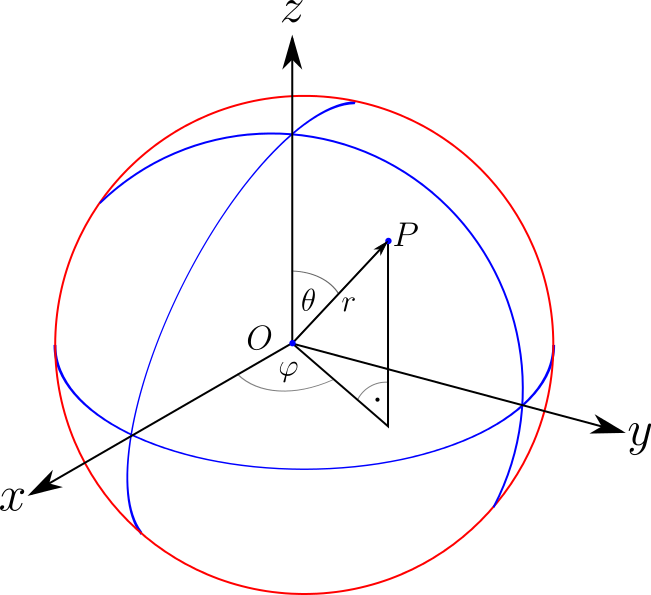
\includegraphics[width=0.75\textwidth]{images/Auswertung/Kugelkoordinaten}
	\caption{Kugelkoordinaten}
	\label{kugelkoordinaten}
\end{figure}



Da dass das Darstellen von Kugelkoordinaten in Matlab nicht ohne weiteres möglich ist, werden die Messwerte in kartesische Koordinaten umgerechnet.
Die Umrechnung erfolgt wie in 

\begin{equation}\formelentry{Umrechung Kugelkoordinaten in kartesische Koordinaten}
	\begin{split}
		&x = r \cdot \cos(\theta) \cdot \cos(\phi) \\
		&y = r \cdot \cos(\theta) \cdot \sin(\phi) \\
		&z = r \cdot \sin(\theta)
	\end{split}
\end{equation} 
\begin{flalign*}
&r = \text{Abstand des Punktes zum Zentrum} \left[m \right]&\\
&\theta = \text{Polarwinkel}\left[^{\circ} \right]&\\
&\phi = \text{Azimutwinkel}\left[^{\circ} \right]&
\end{flalign*}



\begin{lstlisting}[caption={Umwandlung von Kugelkoordinaten zu kartesischen Koordinaten},language={Matlab}, label={import_data}, numbers=left]
for i = 1:1:length(data)
	if(distance(i) < 2000)
		x(i) = -distance(i)*cos(deg2rad(elevation(i)))*cos(deg2rad(azimuth(i)));
		y(i) = distance(i)*cos(deg2rad(elevation(i)))*sin(deg2rad(azimuth(i)));
		z(i) = distance(i)*sin(deg2rad(elevation(i)));
	else
	end
end
\end{lstlisting}


\section{Darstellung der Messwerte}

\begin{lstlisting}[caption={Darstellung der Messwerte},language={Matlab}, label={import_data}, numbers=left]
plot3(x,y,z, '.')
axis([-400 400 -400 400 0 240])
pbaspect([1 1 0.3])
\end{lstlisting}

Rote Punkte
Linien
Kleine Feine Punkte

Standartisierung der Ansicht